\chapter{Gathering information and creating a plan}\label{ch:A}
\section{Brainshtrom and Meetings}
As mentioned earlier, for a long time we could not decide on the topic of our thesis. In this connection, they gathered every weekend live (unfortunately, at that time I did not figure out how to shoot these meetings). We wrote down the ideas of each participant separately and examined them under a microscope. So that we can identify problems that may arise. In most cases, our ideas were successful and were not so difficult to write. But therein lay the problem. We had too much free space because of which our eyes, let's say, ran up. This was the main reason for waiting for topics for graduation theses. We hoped that there would be something close to what we had already come up with and worked out in advance. And, I will not repeat myself, the ideal option has come for us.
\\
All links to our meetings are here \cite{youtube}. After defining the topic of the project, another participant joined us and we met two more times to further distribute tasks among all group members. After that, our meetings were limited to calls from our PM, who followed the process of writing the site and project deadlines.
\section{Plan of project}
At the planning stage of the project, we could not decide which of the methodologies we would use. Our lead PM preferred the waterfall methodology, as the project had a structured flow, with each element following the other. He also suggested supplementing the waterfall with Kanaban to make it easier to follow the project and, in case of any shifts, thanks to a flexible methodology, problems can be responded to and fixed much faster.
\\
Below you can see the Gantt chart that was made by our PM at the beginning of our project \ref{fig:plan1}. The plan and diagram did not change throughout the project. But in the course of the project, thanks to the Kanaban board, additional tasks or additions to the already completed tasks were introduced. Do not forget that every two weeks we had a meeting with {\mycoach}, so the project and its tasks were edited every two weeks.
\\
Also below you can see our Kanban table \ref{fig:knbrd}, in which we followed the process of each member of our team. All the tasks described in it have been approved by our entire team. Accordingly, each of the participants took part in its writing. As mentioned earlier, this table was created so that we can keep track of any deviations in our project or changes that our practice teacher {\mycoach} advised us to make. In particular, you can see the plan that was written on the page of our directory \cite{gitlink}, which describes the detailed work of each of the members of our group \ref{fig:weeksplan}.



\begin{figure}[ht]
    \centering
    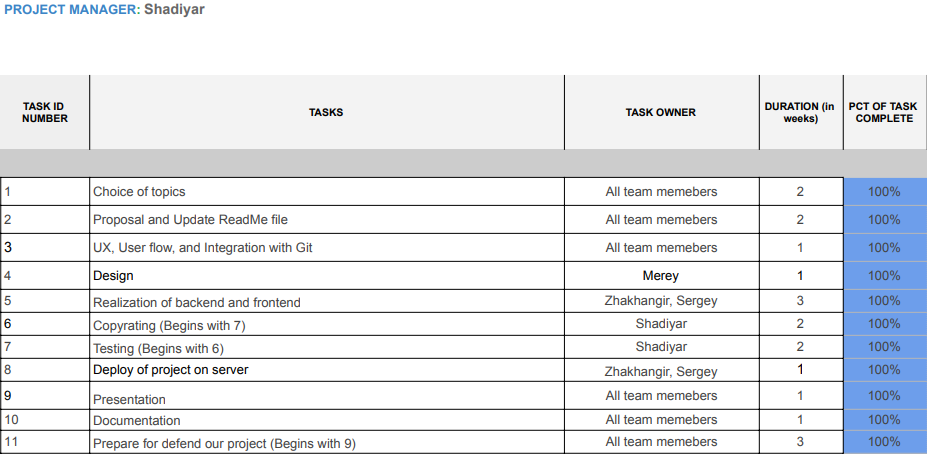
\includegraphics[scale=0.5]{plan1.png}
    \caption{Gantt chart}
    \label{fig:plan1}
\end{figure}

\begin{figure}[ht]
    \centering
    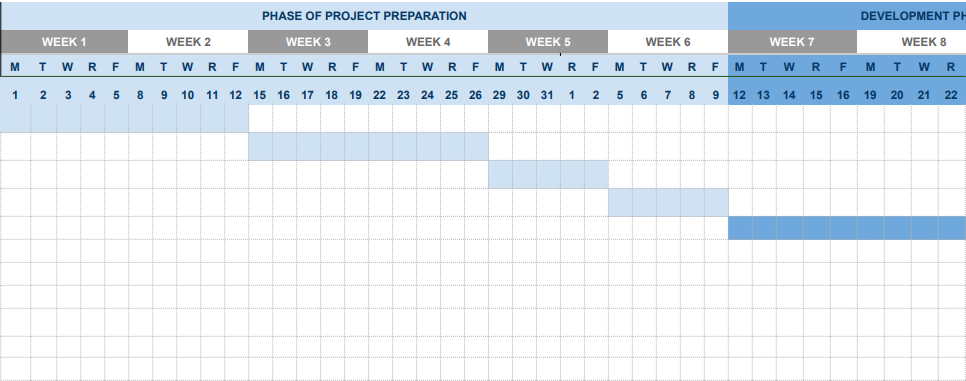
\includegraphics[scale=0.5]{plan2.png}
    \caption{Gantt chart}
    \label{fig:plan2}
\end{figure}

\begin{figure}[ht]
    \centering
    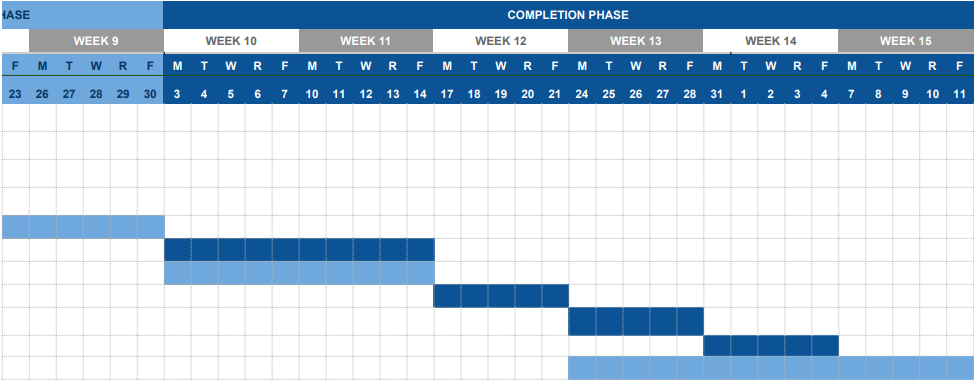
\includegraphics[scale=0.5]{plan3.png}
    \caption{Gantt chart}
    \label{fig:plan3}
\end{figure}

\begin{figure}[ht]
    \centering
    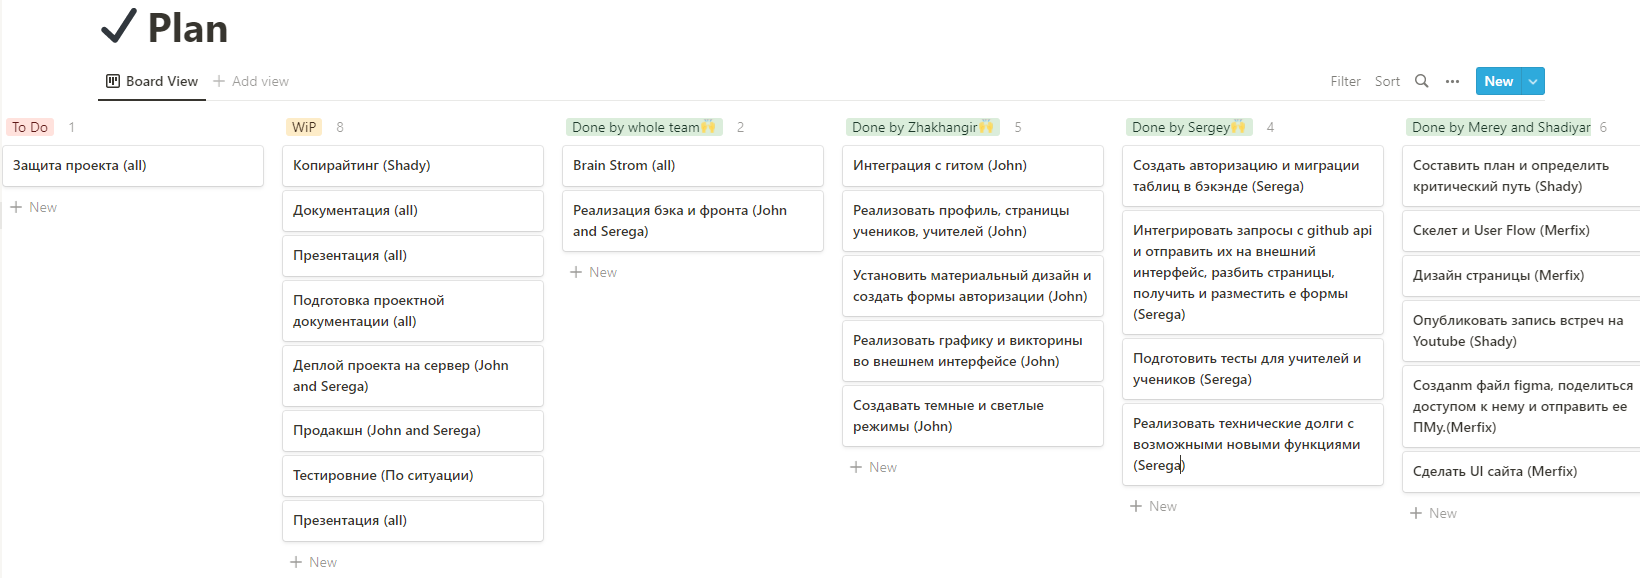
\includegraphics[scale=0.5]{Kanbanbrd.png}
    \caption{Kanban board}
    \label{fig:knbrd}
\end{figure}
%Картинка съезжает, придумать, что с этим делать%
\begin{figure}[t]
    \centering
    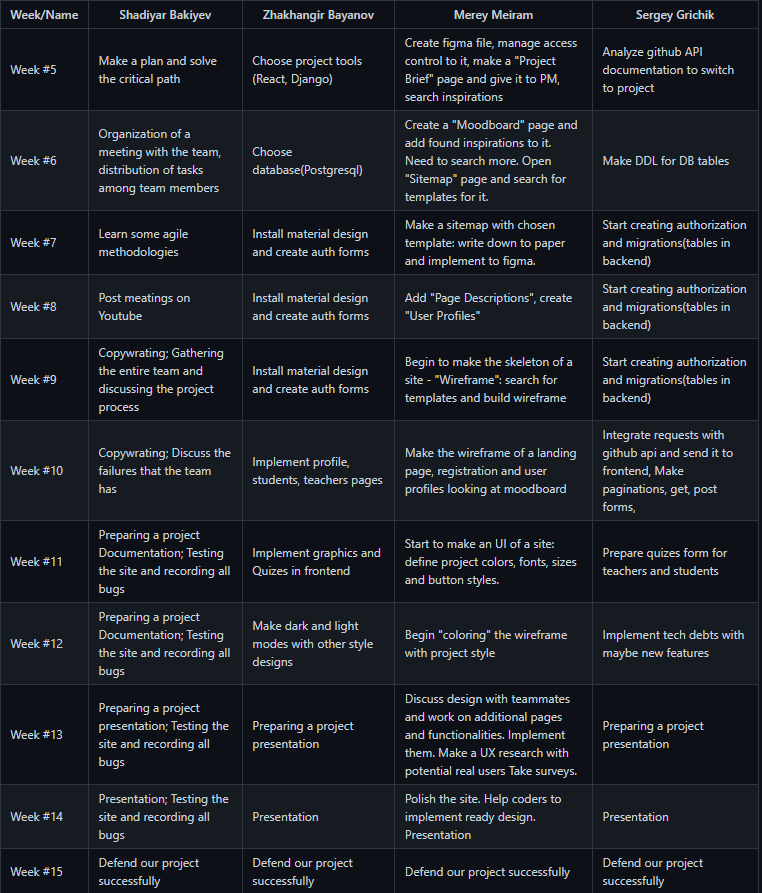
\includegraphics[scale=0.5]{weeksplan.png}
    \caption{Plan on Git}
    \label{fig:weeksplan}
\end{figure}

%\enlargethispage{\baselineskip}
\section{User Personas and Stories}

\section{Sitemap, Page descriptions}
